\subsection{Definition von Emotionen} \label{definition-emotionen}


\todo[inline]{Verantwortlich: Arnaud}


Der Begriff ``Emotion'' wird zwar weltweit  (in fast allen Sprachen) und von alle Menschen verwendet (die soziale oder intellektuelle Ebene spielt keine Rolle), ist aber relativ schwer zu definieren. 
Dieses Paradox wurde bereits im folgenden Zitat explizit erwähnt: 
``Everybody knows what an emotion is, until asked to give a definition.''\cite{fehr_russel_1984} von Fehr und Russell, zwei amerikanischer Emotionsforscher (Psychologe). 
Noch überraschender ist die Schwankung in der Definition dieses Begriffs ``Emotion'' im Laufe der Zeit: Allein die englischsprachige Experimentalpsychologie\cite{plamper12} liefert zwischen 1872 und 1980 mehr als 92 verschiedene Definitionen. 
Wir verstehen daher, dass es schwierig wäre, zu versuchen, diese Definition zu formulieren.  
Wie können wir also die Schwierigkeit, eine Definition für einen solchen gemeinsamen Begriff zu finden, erklären? 
Man sollte nicht vergessen werden, dass es sich um einen eher abstrakten Begriff handelt und daher ist die Emotion sehr subjektiv. 
Neben diesem abstrakten Aspekt ist auch anzumerken, dass sich der Begriff der Emotion auch auf viele Bereiche bezieht, die sich ebenso voneinander unterscheiden wie sie variieren: z.B. Literatur, Philosophie, Psychologie usw. 
Neben diesem multidisziplinären Charakter, der die Pluralität der Vorstellungen und Ansätze in jedem Definitionsversuch erklären könnte, ist es auch notwendig, die Variationen von Sprachen, Perioden und sogar Kulturen hinzuzufügen. \\


Es wird uns allein mit dieser Arbeit (und das ist auch nicht von uns erwartet) nicht möglich sein, alle Fragen im Zusammenhang mit der Definition des Begriffs ``Emotion'' zu betrachten, aber wir werden einige konkrete Beispiele vorstellen, um die Komplexität zu veranschaulichen, die sich aus der Suche nach einer Definition von Emotion ergeben kann.  
Die antiken Philosophen\cite{geslin13} waren die ersten, die sich mit Emotionen und ihren Einflüssen auf den Alltag beschäftigen haben. 
Tatsächlich nahmen Stoiker wie Zeno und Plato bereits 370 n. Chr. Emotionen als eine Krankheit der Seele wahr, die für sie ein Hindernis für denjenigen war, der denken wollte. 
Platon geht mit seiner Allegorie von der Höhle tiefer, indem er alles was emotional ist  mit alle vernünftig (verständlich) kontrastiert: das heiß Emotion und Vernunft gehen nicht zusammen. 
Descartes und Aristoteles vervollständigen Platons Beobachtungen, indem sie in die Analyse von Emotionen eine Dualität (positiv und negativ) der Perzeption einbringen. 
Aristoteles glaubt, dass alles, was das Leben auf positive Weise beeinflusst, durch positive Emotionen bedingt ist, und Descartes glaubt, dass Emotionen für unser Überleben unerlässlich sind und dass die Schwäche eines Menschen eng mit der Fähigkeit der Seele verbunden ist, seine Emotionen zu kontrollieren. 
Charles Darwin in seinem präsentierte weitere ebenso faszinierende neue Elemente über Emotionen, ohne den bisherigen Beobachtungen zu widersprechen\cite{darwin1872}. 
Er verallgemeinert die Emotionen für alle Kulturen und fand sogar ähnlichkeit mit Tiere. 
Der Darwin präsentiert  Emotionen  als Körpersignale (oder Reaktionen) auf äußere Handlungen(Externe Ereignisse), begleitet von spezifischen körperlichen Äußerungen wie: Gesichtsausdrücke, Gesten und oft Geräusche, die alle  spezifisch je nach Emotionen sind. \\


So können wir weiterhin andere berühmte wissenschaftliche Namen wie William James\cite{james1884}, Walter Cannon\cite{cannon32}, Stanley Scharter\cite{schachter59} usw. nennen, die zu unterschiedlichen Zeiten und an unterschiedlichen Orten das Thema untersucht haben, mit ebenso relevanten wie unterschiedlichen Schlussfolgerungen, aber die Beobachtung bleibt die gleiche, die Definition bleibt unbeständig.
Neben den Schwierigkeiten, die sich aus den oben genannten unterschiedlichen Wahrnehmungen ergeben, trägt die  tägliche missbräuchliche Verwendung bestimmter Begriffe wie Gefühl, Affekt, Stimmung, Gefühl (um nur einige zu nennen) als Synonym für Emotionen dazu bei  mehr Verwirrung in das Verständnis von Emotionen. Diese Begriffe beziehen sich zwar auf Gemütszustände, sind aber jedoch nicht Synonym von Emotion\cite{plamper12}.
Trotz des fehlenden Konsenses über die Frage der Definition dieses Begriffs gibt es jedoch Elemente, die in allen Definitionsversuchen wiederkehren, nämlich: 

\begin{itemize} \setlength\itemsep{-0.15cm}
  \item das Vorhandensein eines Auslösers;
  \item den psychischen Zustand des Subjekts;
  \item einen bestimmten Körperausdruck;
  \item eine physiologische Reaktion (Herzfrequenz, Atmung,Schwitzen ...);
  \item eine bestimmte Qualität, Intensität und Dauer.
\end{itemize}


Basierend auf den obigen Elementen können wir daher zu dem Schluss kommen, dass wir zwar nicht genau definieren können, was eine Emotion ist, können wir aber jedoch jede davon mit Bestimmte spezifisch  Element in Verbindung setzen: einen Stimulus (der der Auslöser der Emotion ist), eine physiologische und körperliche Reaktion. 
Die Existenz mehrerer verschiedener Emotionen lässt sich gerade wegen der Spezifität dieser Elemente vermuten. 
Im nächsten Teil werden wir versuchen, die verschiedenen Emotionen zu klassifizieren, mit einem besonderen Fokus auf diejenigen, die wir zu induzieren versuchen. \\


Wie bei der Definition von Emotionen gibt es keine einheitliche Klassifizierung von Emotionen. 
Und wie bei den versuchten Definitionen gab es im Laufe der Zeit mehrere vorgeschlagene Klassifikationen, die sich auch im Laufe der Zeit entwickelt haben. 
Diese Mehrheit von klassifikationen ist vermutlich eine Folge des Mangels an Konsens über die Definition selbst. 
Es gibt jedoch zwei Arten von Klassifikationen, die vor allem unterscheidet und durchgesetzt haben: eine dimensionale Klassifikation\cite{geslin13} und eine kategorische Klassifikation\cite{basic_emotions_theories}.




\subsubsection{Kategoriale Klassifikation} \label{kategoriale-klassifikation}

Angetrieben von Charles Darwin, (der auch der erste war, der grundlegende Emotionen identifizierte) diese Vorgehensweise ist die von Emotionsforscher  mit einer evolutionären Ansatz. 
Diese Klassifikation basiert auf der Existenz von eine Reihe von sogenannten Grundemotionen oder primäre Emotionen. 
Diese  Emotionen wäre in einer begrenzten Anzahl und ihre Entwicklung wurde stark von der Evolution  beeinflusst. 
Wie viele Dinge in Bezug auf die Emotionen in allgemein, variiert die Anzahl von Grundemotionen von einem Emotionsforscher zu einem anderen (siehe Tabelle \ref{vergleich-basisemotionen}).


\begin{table}[h] \centering
\begin{tabular}{| p{5cm} | p{11cm} |}
\hline
\textbf{Forscher} & \textbf{Basisemotionen} \\ \hline
Gray (1982) & Furcht, Freude, Ärger \\ \hline
Panksepp (1982) & Furcht, Erwartung, Ärger, Panik \\  \hline
Tomkins (1984) & Furcht, Freude, Ärger, Verzweiflung, Ekel, Überraschung, Interesse, Scham, Zufriedenheit \\  \hline
Plutchik (1980) & Furcht, Freude, Ärger, Traurigkeit, Ekel, Überraschung, Akzeptanz, Erwartung \\  \hline
Arnold (1960) & Furcht, Liebe, Ärger, Traurigkeit, Hass, Hoffnung, Begehren, Mut, Niedergeschlagenheit, Verzweiflung, Widerwille \\  \hline
Oatley \& Johnson-Laird (1987) & Furcht, Glück, Ärger, Traurigkeit, Ekel \\  \hline
Ekman (1982) & Furcht, Freude, Ärger, Traurigkeit, Ekel, Überraschung \\  \hline
Izard (1987) & Furcht, Freude, Ärger, Traurigkeit, Ekel, Überraschung, Interesse,Verachtung \\ \hline
\end{tabular} \caption[Vergleich einige Basisemotions-Theorien]{ Vergleich einige Basisemotions-Theorien\cite{basic_emotions_theories}. } \label{vergleich-basisemotionen}
\end{table}



Obwohl sie sich nicht über die Anzahl der Grundemotionen einig sind, sind sich die Forscher einig über die Existenz komplexerer Emotionen, die die Kombination mehrerer primärer Emotionen wären. 
Basierend auf diesem Ansatz wurden mehrere Theorien entwickelt, um Emotionen darzustellen, von denen eine der bekannte das Plutchik-Modell ist. 
Plutchiks Modell verwendet ein radförmiges Diagramm (siehe Abbildung \ref{plutchik}) und verschiedene Farben, um jede Emotion darzustellen. \\


\begin{figure}[h]
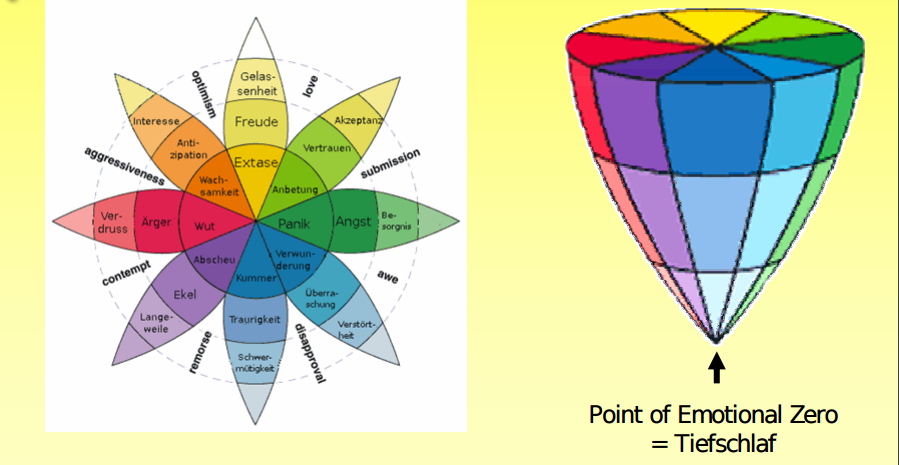
\includegraphics[width=\textwidth]{Images/plutchik.png} 
\vspace{-0.3cm} 
\caption{ Einordnung von Emotion nach Plutchik. }
\label{plutchik} 
\end{figure}


Diese Theorie fundiert sich auf  das acht primäre Emotionen mit einer klare trennung (bzw unterschied) zwischen  primären, sekundären und tertiären Emotionen.
Die verbindet jede primäre Emotion mit spezifischen Motivationssystem und Verhaltendstedenze zur Bewältigung grundlegender adaptiver Probleme (siehe Tabelle \ref{verhalten-funktion}). 


\begin{table}[h] \centering
\begin{tabular}{| p{5.1cm} | p{5.1cm} | p{5.1cm} |}
\hline
\textbf{Subjektiv} & \textbf{Verhalten} & \textbf{Funktion} \\ \hline
Angst, Entsetzen & Rückzug, Flucht  & Schutz \\ \hline
Ärger, Wut & Angriff, Beißen & Zerstörung \\ \hline
Freude, Ekstase & Paarung, Besitz & ergreifen Fortpflanzung \\ \hline
Traurigkeit, Trauer & Weinen, Bitte um Hilfe & Reintegration \\ \hline
Akzeptanz, Anbetung, Vertrauen & Paarbildung, Pflege & Zusammengehörigkeit, Bindung \\ \hline
Ekel, Abscheu & Sich übergeben & Ablehnung, Zurückweisung \\ \hline
Erwartung, Antizipation & Untersuchen & Exploration, Erkundung \\ \hline
Überraschung & Innehalten, Einfrieren & Orientierung \\ \hline
\end{tabular} \caption[ Einige Basisemotionen jeweils mit Verhalten und Funktio ]{ Einige Basisemotionen jeweils mit Verhalten und Funktion\cite{basic_emotions_theories}. } \label{verhalten-funktion}
\end{table}






\subsubsection{Kategoriale Ansatz} \label{kategoriale-ansatz}

Dieser von Wundt\cite{basic_emotions_theories} initiierte Ansatz geht von dem Gedanken aus, dass die emotionale Erfahrung in einem mehrdimensionalen Raum dargestellt werden kann. 
Dieser Zerlegung der emotionale Erfahrung  sollte es ermöglichen, eine genaue Analogie zwischen Emotion und Körperausdruck (Gesichtsausdrücke) herzustellen. 
Dieser Ansatz wurde  daher den Vorteil, dass sie die Tür zu einer möglichen Quantifizierung der emotionalen Erfahrung öffnet. 
Die Idee von Wundt (siehe Abbildung \ref{wundt})  war einer dreidimensionalen Zerlegung(Lust-Unlust, Spannung-Entspannung (Lösung), Beruhigung (Ruhe)-Erregung siehe) der emotionalen Erfahrung. 


\begin{figure}[h]
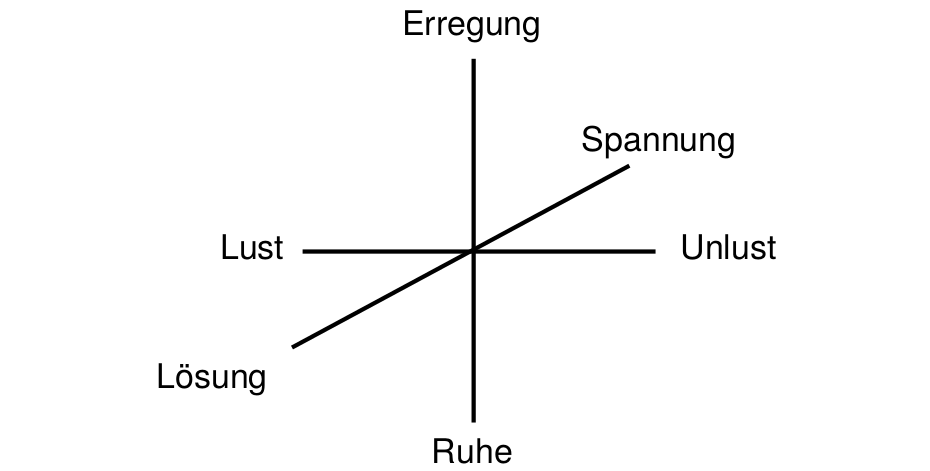
\includegraphics[width=\textwidth]{Images/wundt.png} 
\vspace{-0.3cm} 
\caption[Einordnung von emotionale Erfahrungsprozess nach Wundt.]{ Einordnung von emotionale Erfahrungsprozess nach Wundt\cite{basic_emotions_theories}. }
\label{wundt} 
\end{figure}


Die Frage nach der Anzahl der Dimensionen, die zur Darstellung der emotionalen Erfahrung notwendig sind, wird jedoch zu mehreren Theorien führen. 
Allerdings schlug Russell\cite{basic_emotions_theories} eine zweidimensionale Darstellung mit sechs primären Emotionen nach Ekam vor (siehe Tabelle \ref{vergleich-basisemotionen}). 
Emotionen werden also dank dieses Modells (siehe Abbildung \ref{russell}) eine horizontale Komponente haben: Valenz (Freude/Verdruss) und eine vertikale Komponente: Erregung (Aktivierung). 


\begin{figure}[h] \centering
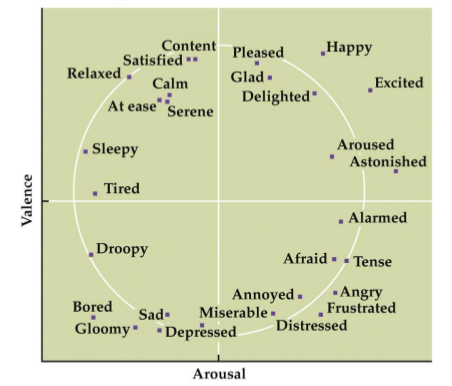
\includegraphics[width=12cm]{Images/russell.png} 
\vspace{-0.3cm} 
\caption[Einordnung von emotional Erfahrung nach Russell.]{ Einordnung von emotional Erfahrung nach Russell\cite{basic_emotions_theories}. }
\label{russell} 
\end{figure}


Die Valenz unterscheidet positive Emotionen von negative Emotionen, und die Erregung informiert über körperliche Erregung, die man durch die Anzahl von physiologischen Reaktion feststellen kann. 
Jede Emotion lässt sich als Kombination dieser beiden Parameter darstellen was für eine mathematische auswertung sehr hilfreich sein könnte. 
Dieses Modell hat viel Erfolg gehabt, da er die Darstellung von eine Unendlichkeit von Emotionen erlaubt hat. 
Trotz der unterschiedlichen Anzahl von Dimensionen von verschiedenen Autoren vorgeschlagen, die beiden Dimensionen von Russell (Valenz und Erregung) sind Faktoren die in fast alle Modelle dieses Ansatzes auftreten.



